% $File: report.tex
% $Date: Mon Dec 30 22:21:17 2013 +0800
%Author: Yuxin Wu <ppwwyyxxc@gmail.com>

\documentclass {beamer}
%\usetheme{JuanLesPins}
\usetheme{Copenhagen}
\setbeamertemplate{itemize items}[ball]
\setbeamercovered{transparent}
\setbeamertemplate{itemize subitem}[circle] % if you wnat a circle
\setbeamertemplate{blocks}[rounded][shadow=true]
%\usetheme[height=7mm]{Rochester}
\useoutertheme{infolines}
\usepackage{fontspec,amsmath,amssymb,zhspacing,verbatim}
\usepackage[backend=biber]{biblatex}


\let\Oldsum\sum
\renewcommand{\sum}{\displaystyle\Oldsum}
\let\Oldprod\prod
\renewcommand{\prod}{\displaystyle\Oldprod}

\theoremstyle{plain}

\usepackage[absolute,overlay]{textpos}
\newenvironment{reference}[2]{%
  \begin{textblock*}{\textwidth}(#1,#2)
      \footnotesize\it\bgroup\color{red!50!black}}{\egroup\end{textblock*}}

\zhspacing

\setbeamertemplate{footline} {
  \leavevmode%
  \hbox{%
    \begin{beamercolorbox}[wd=\paperwidth,ht=2.25ex]{corporatecolor}
      \begin{beamercolorbox}[wd=.333333\paperwidth,ht=2.25ex,dp=1ex,center]{author in head/foot}%
        \usebeamerfont{author in head/foot}
        \insertshortauthor
      \end{beamercolorbox}%
      \begin{beamercolorbox}[wd=.333333\paperwidth,ht=2.25ex,dp=1ex,center]{title in head/foot}%
        \usebeamerfont{title in head/foot}
        \insertshorttitle
      \end{beamercolorbox}%
      \begin{beamercolorbox}[wd=.333333\paperwidth,ht=2.25ex,dp=1ex,right]{date in head/foot}%
        \usebeamerfont{date in head/foot}\insertshortdate{}\hspace*{2em}
        \insertframenumber{} / \inserttotalframenumber\hspace*{2ex}
      \end{beamercolorbox}
    \end{beamercolorbox}
  }%
  \vskip0pt%
}

\title{Speaker Recognition}
\subtitle{SRT project of Signal Processing}
\author {Xinyu Zhou, Yuxin Wu, Tiezheng Li}
\institute{
  Department of Computer Science and Technology\\
  Tsinghua University\\
}
\date{\today}

\begin{document}

\frame[plain]{\titlepage}

\begin{frame}{Overview}
\tableofcontents
\end{frame}

%File: VAD.tex
%Date: Tue Dec 31 01:12:04 2013 +0800
%Author: Yuxin Wu <ppwwyyxxc@gmail.com>

\section{VAD}
\begin{frame}{VAD}
  \textbf{Voice Activity Detection} shall be applied for all signals as a pre-filter.
  We've tried 2 different approaches:
  \pause
  \begin{itemize}
    \item Energy-Based:
      \begin{itemize}
        \item Filter out the intervals with relatively low energy.
        \item Work perfectly for high-quality recordings.
        \item Sensitive to noise.
      \end{itemize}
      \pause

    \item Long-Term Spectral Divergence
      \begin{itemize}
        \item Compare long-term spectral envelope with noise spectrum.
        \item More robust to noise, used in our GUI.
        \item
            \footnotesize\it\color{red!50!black}
            Efficient voice activity detection algorithms using long-term speech information,
            Ramırez, Javier, 2004
      \end{itemize}
  \end{itemize}
\end{frame}

\begin{frame}{LTSD}
  \begin{center}
    \includegraphics[width=0.7\textwidth]{res/ltsd.png}
  \end{center}
\end{frame}

%File: features.tex
%Date: Mon Dec 30 19:25:01 2013 +0800



\section{Features}
\subsection{MFCC}
\begin{frame}[label=mfcc]{MFCC}
  \textbf{Mel-Frequency Cepstral Coefficients}

  Cepstral feature which closely approximates human auditory system's response.
  Commonly used feature for Speech/Speaker Recognition.
\begin{center}
  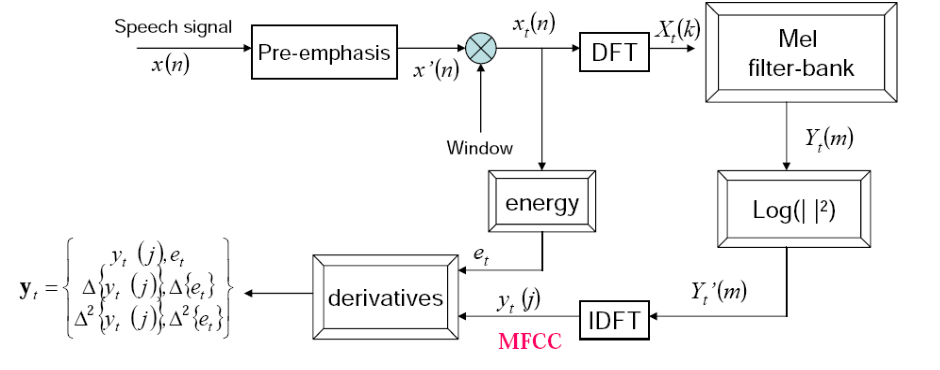
\includegraphics[width=\textwidth]{res/MFCC.png}
\end{center}
\end{frame}

\begin{frame}{Windowing}
\begin{center}
  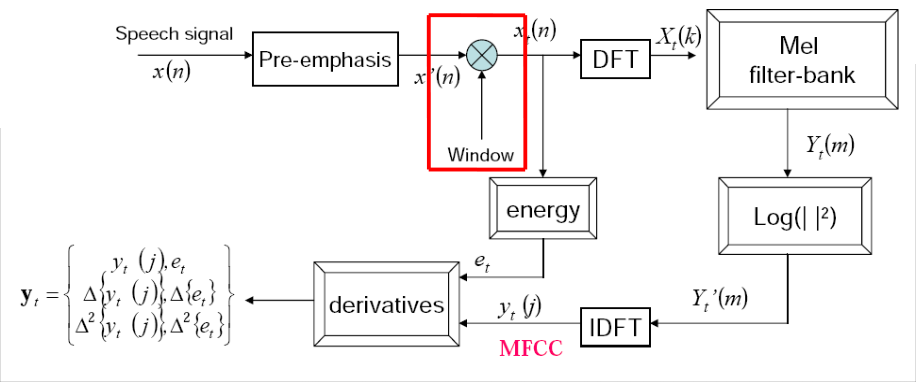
\includegraphics[width=0.6\textwidth]{res/MFCC-windowing.png}\\
  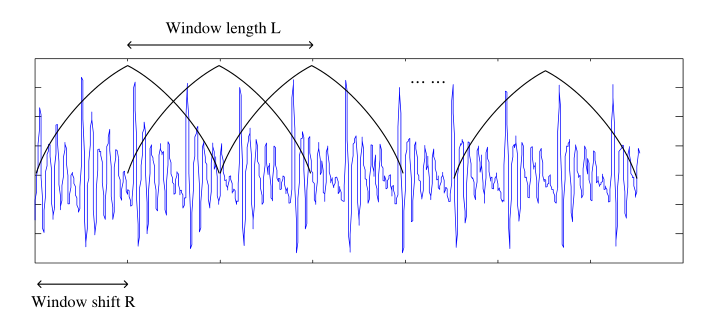
\includegraphics[width=0.8\textwidth]{res/MFCC-windowing-frames.png}
\end{center}
\end{frame}

\begin{frame}{Mel-Scale}
\begin{center}
  \includegraphics[width=0.6\textwidth]{res/MFCC-mel-filterbank.png}
\end{center}
\begin{columns}
  \begin{column}{0.5\textwidth}
    \[ Mel(f) = 2595 \log_{10}(1 + \dfrac{f}{700})\]
  \end{column}
  \begin{column}{0.5\textwidth}
    \begin{flushleft}
      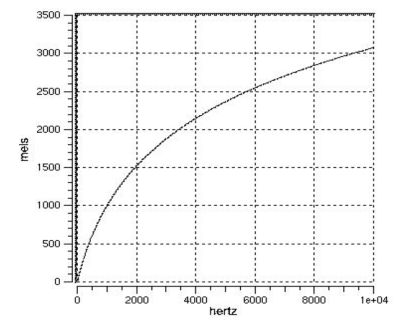
\includegraphics[width=0.7\textwidth]{res/mel-scale.png}
    \end{flushleft}
  \end{column}
\end{columns}
\end{frame}
\againframe{mfcc}


\subsection{LPC}
\begin{frame}{LPC}
  \textbf{Linear Predictive Coding/Coefficients}

\begin{exampleblock}{Assumption}
    In a short period, the $n$th signal is a linear combination of previous $p$ signals:
    $ \hat{x}(n) = \sum_{i=1}^pa_i x(n-i)$
\end{exampleblock}
\pause
Minimize squared error $\text{E}\left[ \hat{x}(n) - x(n)\right] $ using Levinson-Durbin algorithm.

Use $a_1, \cdots  , a_p$ as features.
\end{frame}

\subsection{Experiments on Features}
\begin{frame}{MFCC Params}
\begin{columns}[t]
  \begin{column}[t]{0.5\textwidth}
    \begin{center}
    \includegraphics[width=0.8\textwidth]{res/mfcc-nceps.pdf}\\
    \includegraphics[width=0.8\textwidth]{res/mfcc-frame-len.pdf}
  \end{center}
  \end{column}
  \begin{column}[t]{0.5\textwidth}
    \begin{center}
    \includegraphics[width=0.8\textwidth]{res/mfcc-nfilter.pdf}\\
    Best parameters in our cases:

    Number of cepstrals: 15

    Number of filters: 55

    Frame length: 32ms
  \end{center}
  \end{column}
\end{columns}
\end{frame}

\begin{frame}{LPC Params}
  \begin{center}
    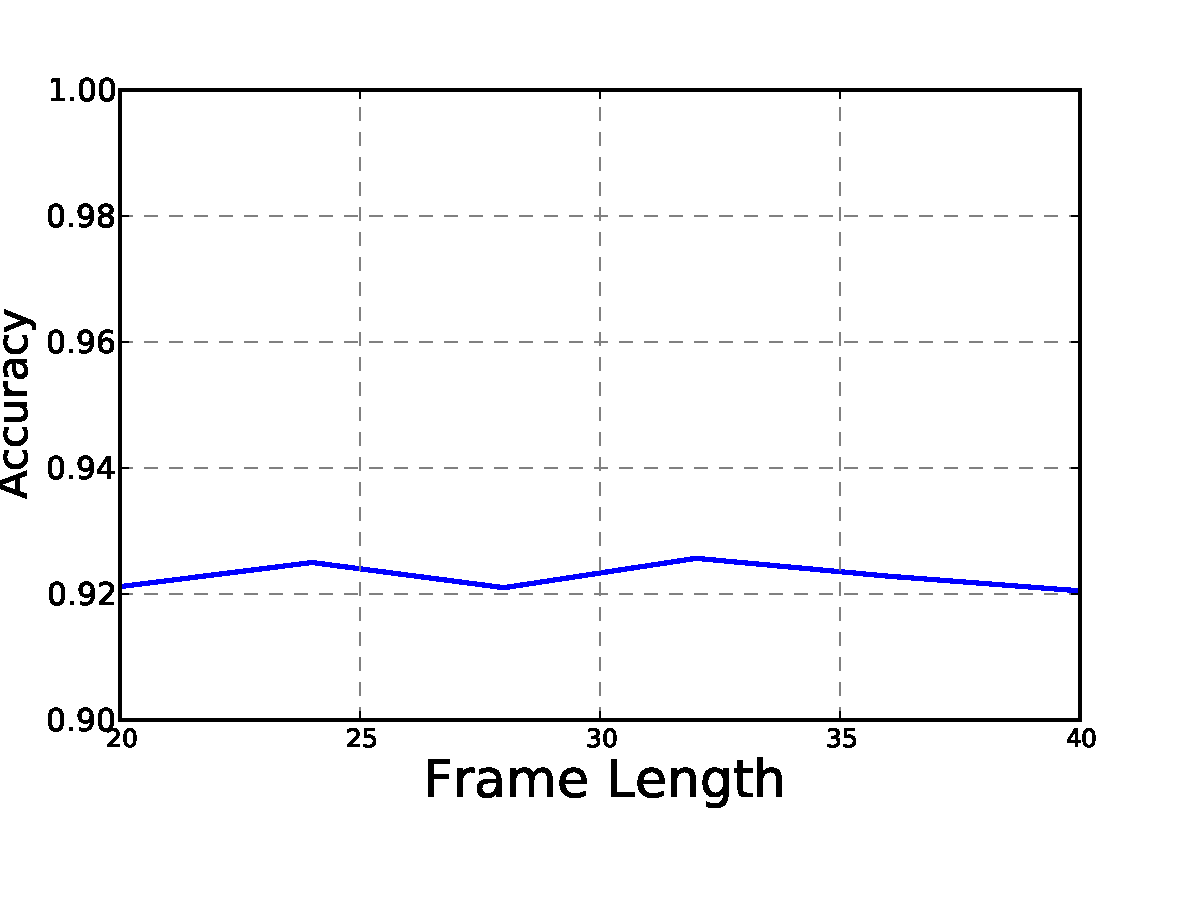
\includegraphics[width=0.5\textwidth]{res/lpc-frame-len.pdf}
    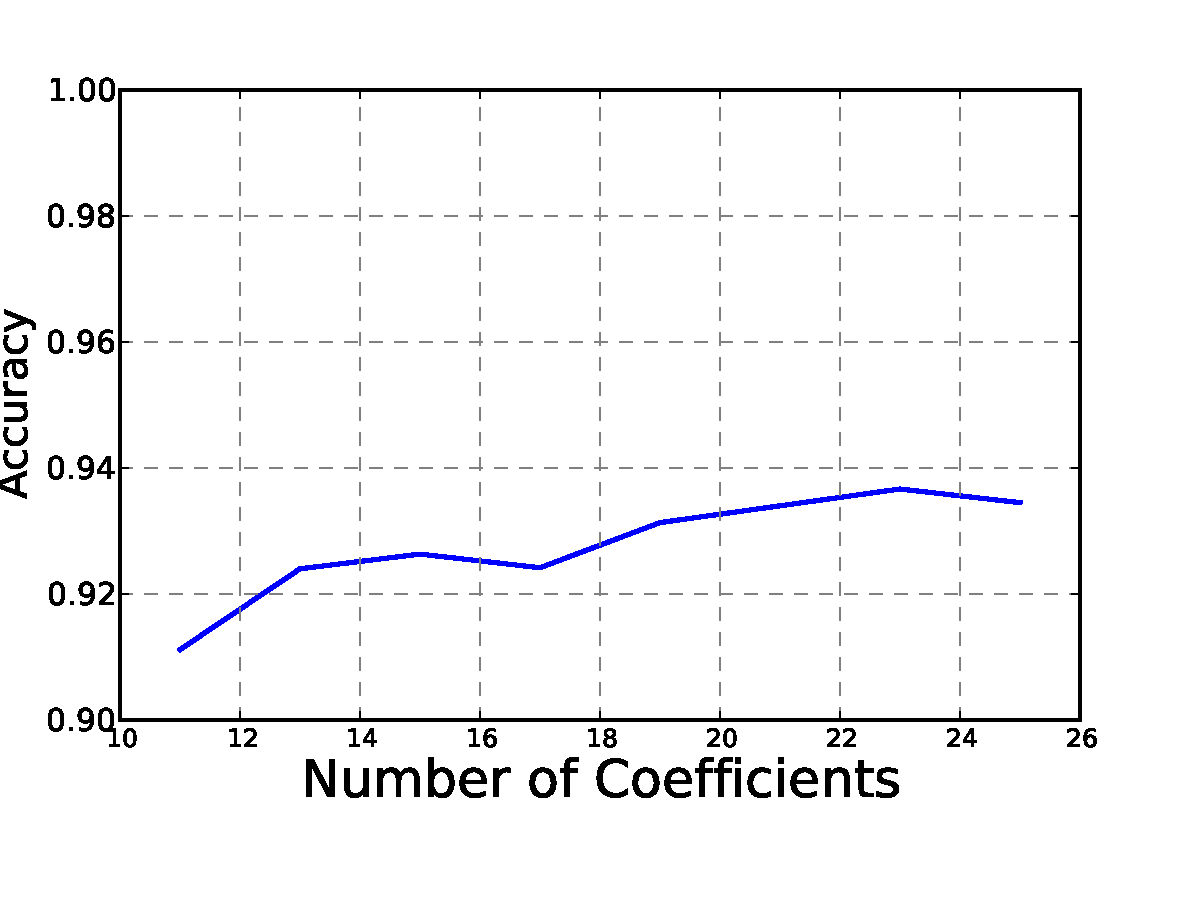
\includegraphics[width=0.5\textwidth]{res/lpc-nceps.pdf}\\
    Best parameter in our cases:

    Number of coefficients: 23

    Frame length: 32ms
  \end{center}
\end{frame}

\section{Model}
%File: GMM.tex
%Date: Fri Jan 03 17:55:16 2014 +0800


\subsection{GMM-UBM}

\begin{frame}{GMM}
  \textbf{Gaussian Mixture Model}
  is commonly used to model human's acoustic feature.  \begin{exampleblock}{}
    \[ p(\theta) = \sum_{i=1}^{K}{w_i \mathcal{N}(\mathbf{\mu}_i, \Sigma_i)}\]
  \end{exampleblock}
  \pause

  \begin{columns}
    \begin{column}{0.5\textwidth}
      \begin{center}
        \only<1>{\includegraphics[width=\textwidth]{res/gmm.png}}
        \visible<2>{ 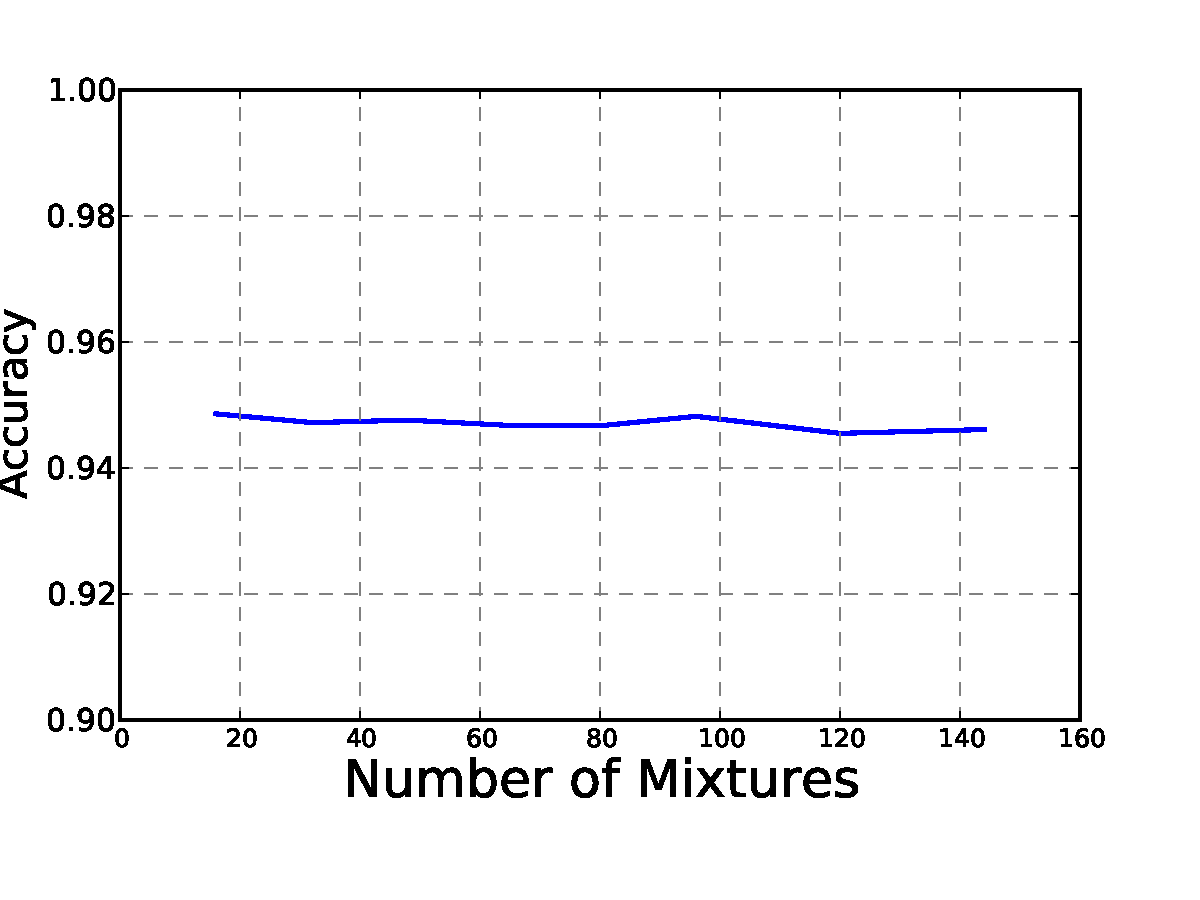
\includegraphics[width=\textwidth]{res/nmixture.pdf} }
      \end{center}
    \end{column}
    \begin{column}{0.3\textwidth}
      We use $ K=32$
    \end{column}
  \end{columns}
\end{frame}

\begin{frame}{Optimized GMM}
  \begin{itemize}
    \item Basic GMM training: random initialize, estimate parameters with EM.
    \item Improvment: initialize with a parallel KMeansII.
    \item Improvment: parallel training implementation in C++.
    \item Compared to GMM from scikit-learn:
  \end{itemize}

  \begin{columns}
    \begin{column}{0.5\textwidth}
      \begin{center}
        \visible<2>{ 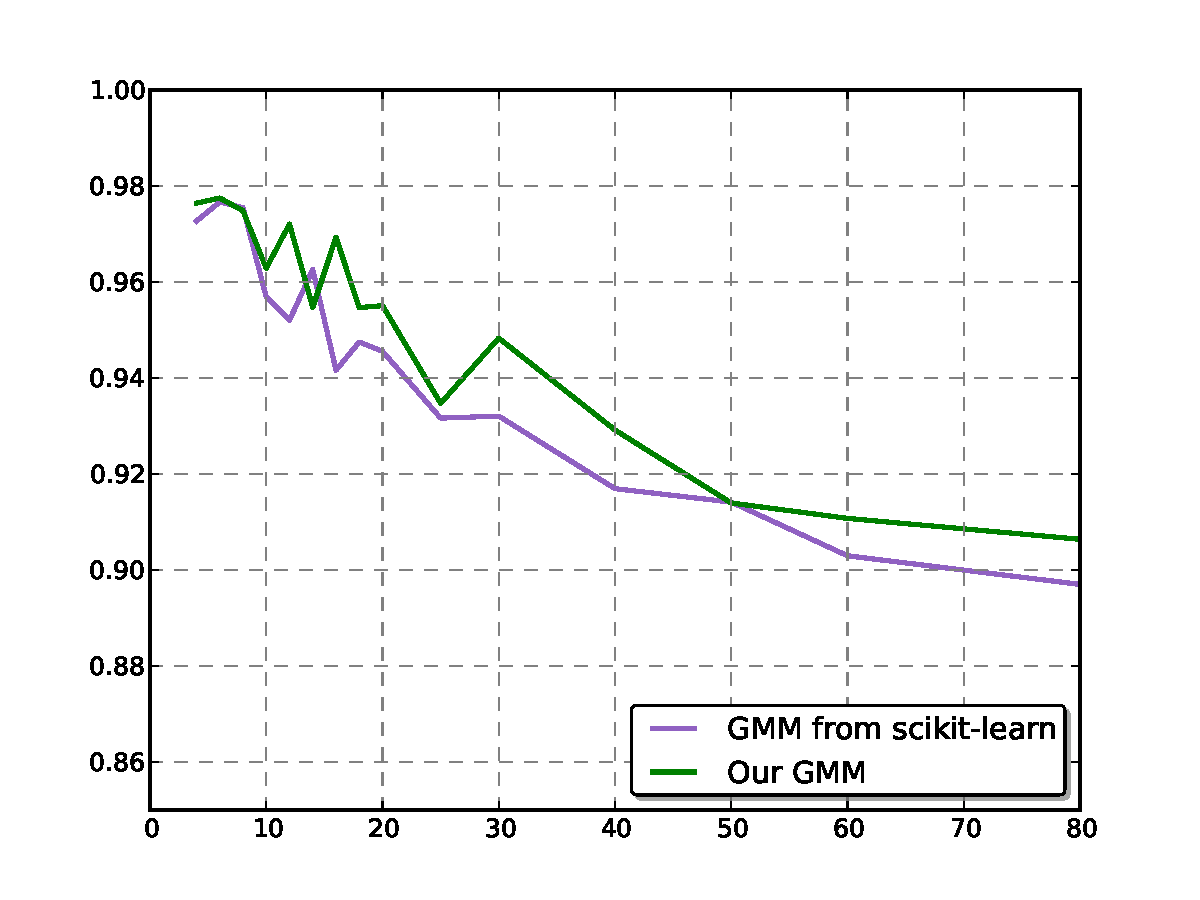
\includegraphics[width=\textwidth]{res/gmm-compare.pdf} }
      \end{center}
      \vspace{0.6em}
    \end{column}
    \begin{column}{0.6\textwidth}
      \visible<2>{ \includegraphics[width=\textwidth]{res/time-comp-small.pdf} }
    \end{column}
  \end{columns}
  \vspace{3em}

  \begin{reference}{4mm}{85mm}
    Arthur, David, Sergei, 2007,
    k-means++: The advantages of careful seeding.

    Bahmani, et. al, 2012,
    Scalable K-means++
  \end{reference}
\end{frame}

\begin{frame}{UBM}
  \textbf{Universal Background Model} is a GMM trained on giant datasets.

  UBM can be used to:
  \begin{itemize}
    \item Describe general acoustic feature of human.
    \item Reject the decision of GMM.
    \item Train adaptive GMM.
  \end{itemize}

  \begin{reference}{4mm}{85mm}
    Reynolds, Douglas, et al, 2000,

    Speaker verification using adapted Gaussian mixture models
  \end{reference}
\end{frame}


\begin{frame}{GMM Results}
  \begin{columns}[t]
    \begin{column}[t]{0.5\textwidth}
      \begin{center}
        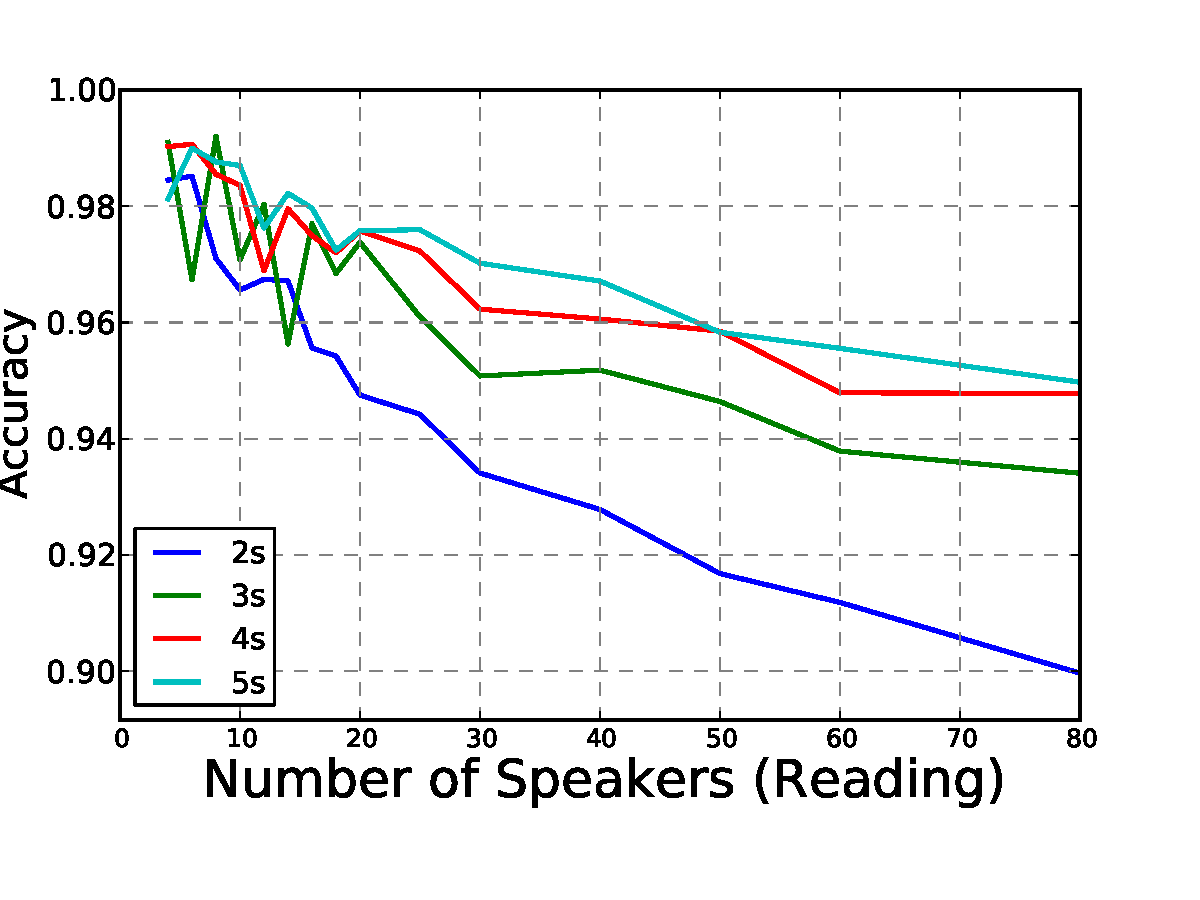
\includegraphics[width=0.8\textwidth]{res/reading.pdf}\\
        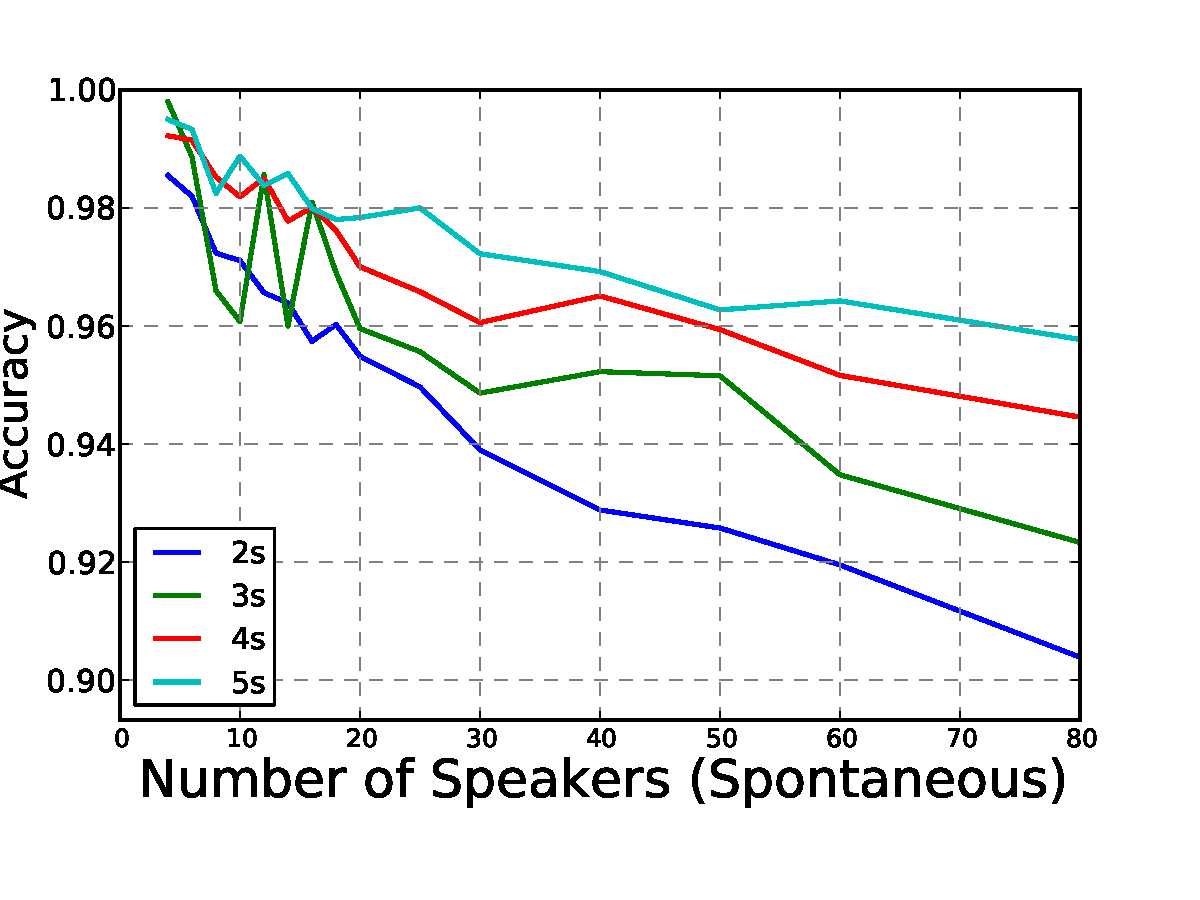
\includegraphics[width=0.8\textwidth]{res/spont.pdf}
      \end{center}
    \end{column}
    \begin{column}[t]{0.5\textwidth}
      \begin{center}
        \includegraphics[width=0.8\textwidth]{res/whisper.pdf}\\
        Train duration: 20s

        Random selected test utterance: 50

        Each value in the graph is an average of 20 independent experiments.
      \end{center}
    \end{column}
  \end{columns}
\end{frame}

%File: RBM.tex
%Date: Mon Dec 30 21:12:54 2013 +0800
%Author: Yuxin Wu <ppwwyyxxc@gmail.com>


\subsection{CRBM}

\begin{frame}{CRBM}
  \begin{itemize}
    \item \textbf{Restricted Boltzmann Machine} is a generative stochastic two-layer neural network.

    \item \textbf{Continuous RBM} extends RBM to real-valued inputs.
      \pause
    \item RBM has a ability to reconstruct a layer similar to input layer.
      The difference between the two layers can be a used to measure the fitness of an input to the model.

    \item Therefore, RBM can be a substituion to GMM.
  \end{itemize}


  \begin{reference}{4mm}{85mm}
Chen, Hsin and Murray, Alan F, 2003,
Continuous restricted Boltzmann machine with an implementable training algorithm
  \end{reference}
\end{frame}

\begin{frame}{Results}
  Results of CRBM, tested with 5 secs
  of utterance.
  \begin{center}
    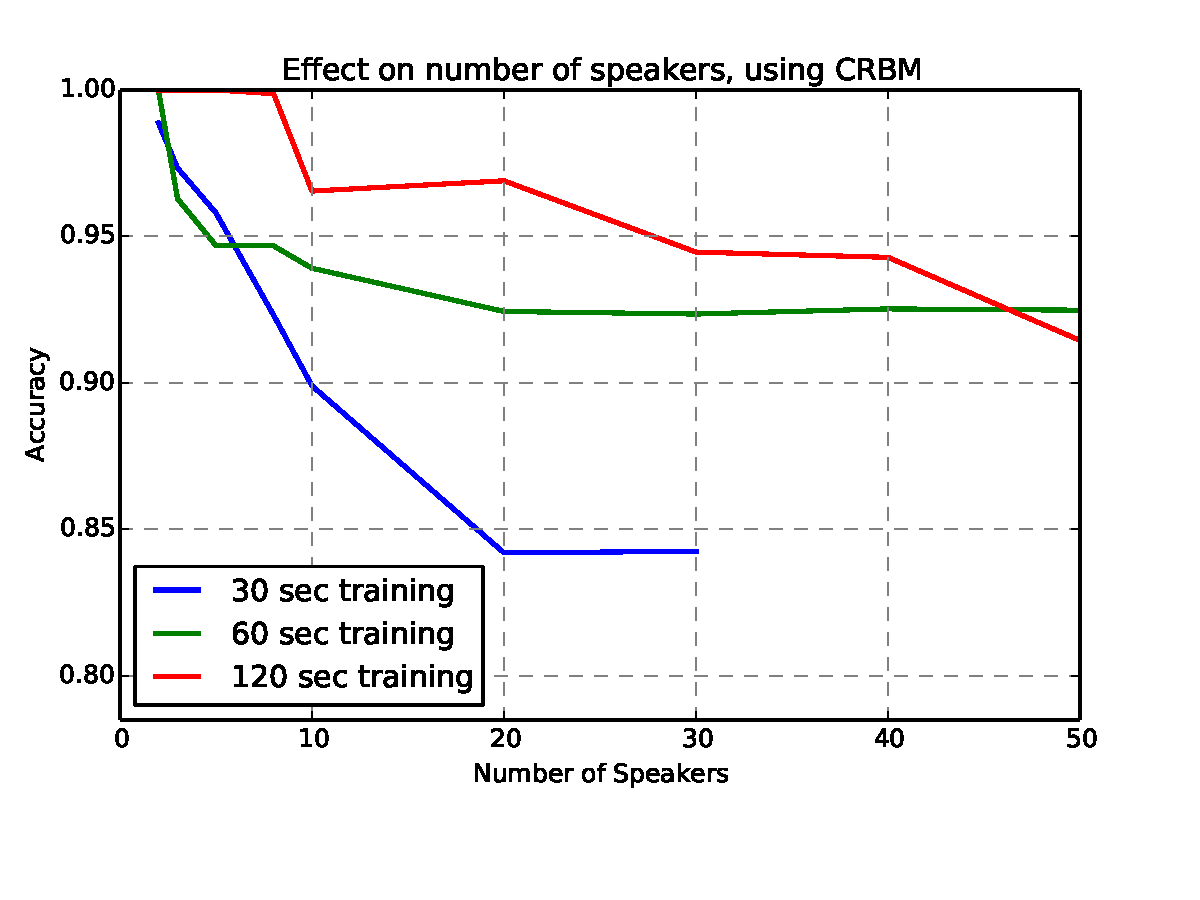
\includegraphics[width=0.7\textwidth]{res/crbm.pdf}
  \end{center}
\end{frame}


%File: JFA.tex
%Date: Mon Dec 30 21:35:32 2013 +0800
%Author: Yuxin Wu <ppwwyyxxc@gmail.com>

\subsection{JFA}

\begin{frame}{JFA}
  \begin{itemize}
    \item \textbf{Factor Analysis} is a statistical method to describe \textbf{variability}
      among observed variables and unobserved variables (factors).

    \item Joint Factor Analysis is a new Speaker Recognition method, taking
      Inter-Channel variability and inter-speaker variability into account.

  \end{itemize}

\end{frame}

\begin{frame}{GUI Demo}

\end{frame}

\end{document}

